\chapter{Introduction}

Video games are a popular form of entertainment.
There is a plethora of games to choose from, each offering a different experience.
Still, it is always possible to create something new that players might enjoy.
The author of this thesis enjoys both \emph{tower defense} games and \emph{roguelike} games and there are not many games that combine these two genres.
In this thesis, we will design and implement a video game, that uniquely blends them, and discuss the decisions behind it.
So, what do we mean by a \emph{roguelike tower~defense} game?

\section{Tower Defense}

A game genre can encompass many characteristics, most often its mechanics, but also its theme, art style or the medium it is played on.
Genres have no exact definitions or strict boundaries, they are characterized by how people use them to describe games.

\textbf{Tower defense} is often described~\cite{TDWiki}\cite{CITD} as a subgenre of \emph{real-time strategy}.
This means the game focuses on long-term planning, but also quick thinking.
In \emph{tower defense} games, the player has to defend against waves of attackers by building defensive towers.
As an example we'll look at \emph{Plants vs.\ Zombies}~\cite{PvZWeb}, released in~2009.

In \emph{Plants vs.\ Zombies}, the player defends their house from zombies.
As shown figure \ref{fig:pvz-fight}, the zombies come from the right side of the screen and advance left.
If any zombie reaches the far left edge of the screen, the player loses the level.
The goal of each level is to survive all the incoming waves by placing plants that kill or otherwise impede the zombies.
We can also see two \emph{Repeaters} in the upper left part of the image, one of them shooting at a zombie.
Further to the left, there are a lot of \emph{Sunflowers}.
These are a very important part of the game, because all plants cost~\emph{sun}, and \emph{Sunflowers} produce those.

\begin{center}
    \captionsetup{type=figure}
    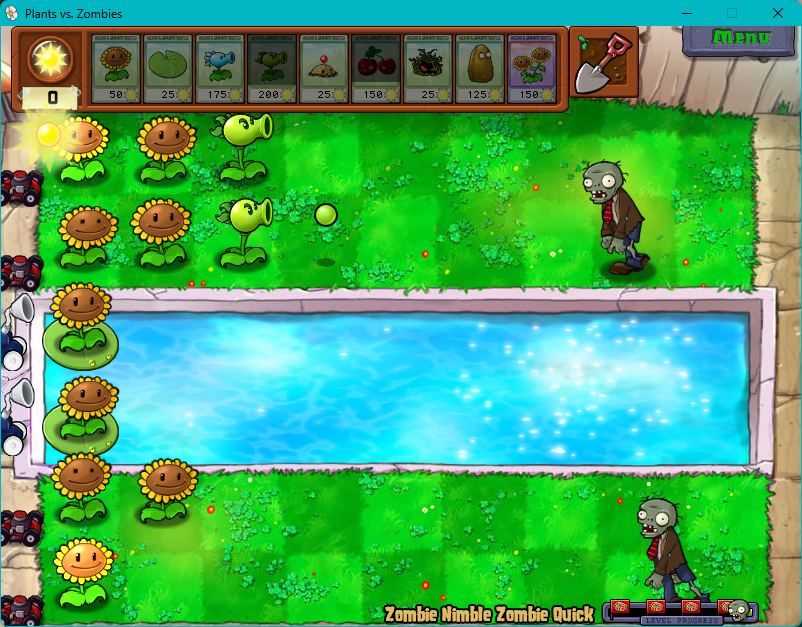
\includegraphics[width=0.8\textwidth]{img/Plants-vs-Zombies-Fight.png}
    \caption{A level in \emph{Plants vs.\ Zombies}.}
    \label{fig:pvz-fight}
\end{center}

In our game, the player will also build towers, to defend from waves of attackers, and economic buildings that produce materials.
Though, it will differ a lot from \emph{Plants vs.\ Zombies} in the overall structure of the game.
The main game mode of \emph{Plants vs.\ Zombies} is a campaign consisting of~50 individual levels.
If the player loses a level, they can try again and~again until they succeed in beating it.
After most levels, the player unlocks a new plant, which they can use in upcoming levels, slowly building up their arsenal.
In our game, however, once the player loses, they lose all their progress and must start from the very beginning.
This and some other mechanics are taken directly from the \emph{roguelike} genre.

\section{Roguelike}

\textbf{Roguelike} is a subgenre of \emph{role-playing games}.
In \emph{role-playing games}, the player takes on the role of a character and goes on an adventure.
The character can grow stronger by acquiring new abilities, items, or~experiences.
The player has to make decisions about how to upgrade their characters to overcome the challenges they might face.
\emph{Role-playing games} are a very broad genre with a long history, for more information we recommend the book \citetitle{rpgBycer}~\cite{rpgBycer} by J.~Bycer.

The \emph{roguelike} genre is named after the game \emph{Rogue}~\cite{RogueWiki}, released in~1980.
In this single-player turn-based game, the player explores a grid-based dungeon and fights monsters that inhabit~it.
Along the way, they collect various weapons, armor and other magical items that improve their abilities.
It features a mechanic nicknamed \emph{permadeath}, which means that when the character dies, the player loses all progress and must start from the very beginning.
The dungeon is randomized~--- it is different in every run, so the player can't just memorize the layout.
These are the most defining features of \emph{roguelikes}, but games of this genre aren't just clones of the original \emph{Rogue}.
The breadth of \emph{roguelike} games is well explored and explained by J.~Bycer~\cite{roguelikeBycer}.

A more recent game that's a good example of this genre is \emph{Slay the Spire}~\cite{StS}.
In \emph{Slay the Spire}, the player ascends a spire and fights various enemies.
The fights are also turn-based, and when the player's character dies, they have to start from scratch.
However, it is not a traditional \emph{roguelike}.
The game is not played on a grid, instead the spire the player navigates is~a graph of separate rooms, where they move from bottom up.
We can see this in figure~\ref{fig:sts-map}.
Here, the player has been to the rooms that are circled, and now they have to choose where to go next.
The player can come across different kinds of rooms, each represented with an icon.
The most important are enemy encounters, where the player fights monsters using a deck of cards.

\begin{center}
    \captionsetup{type=figure}
    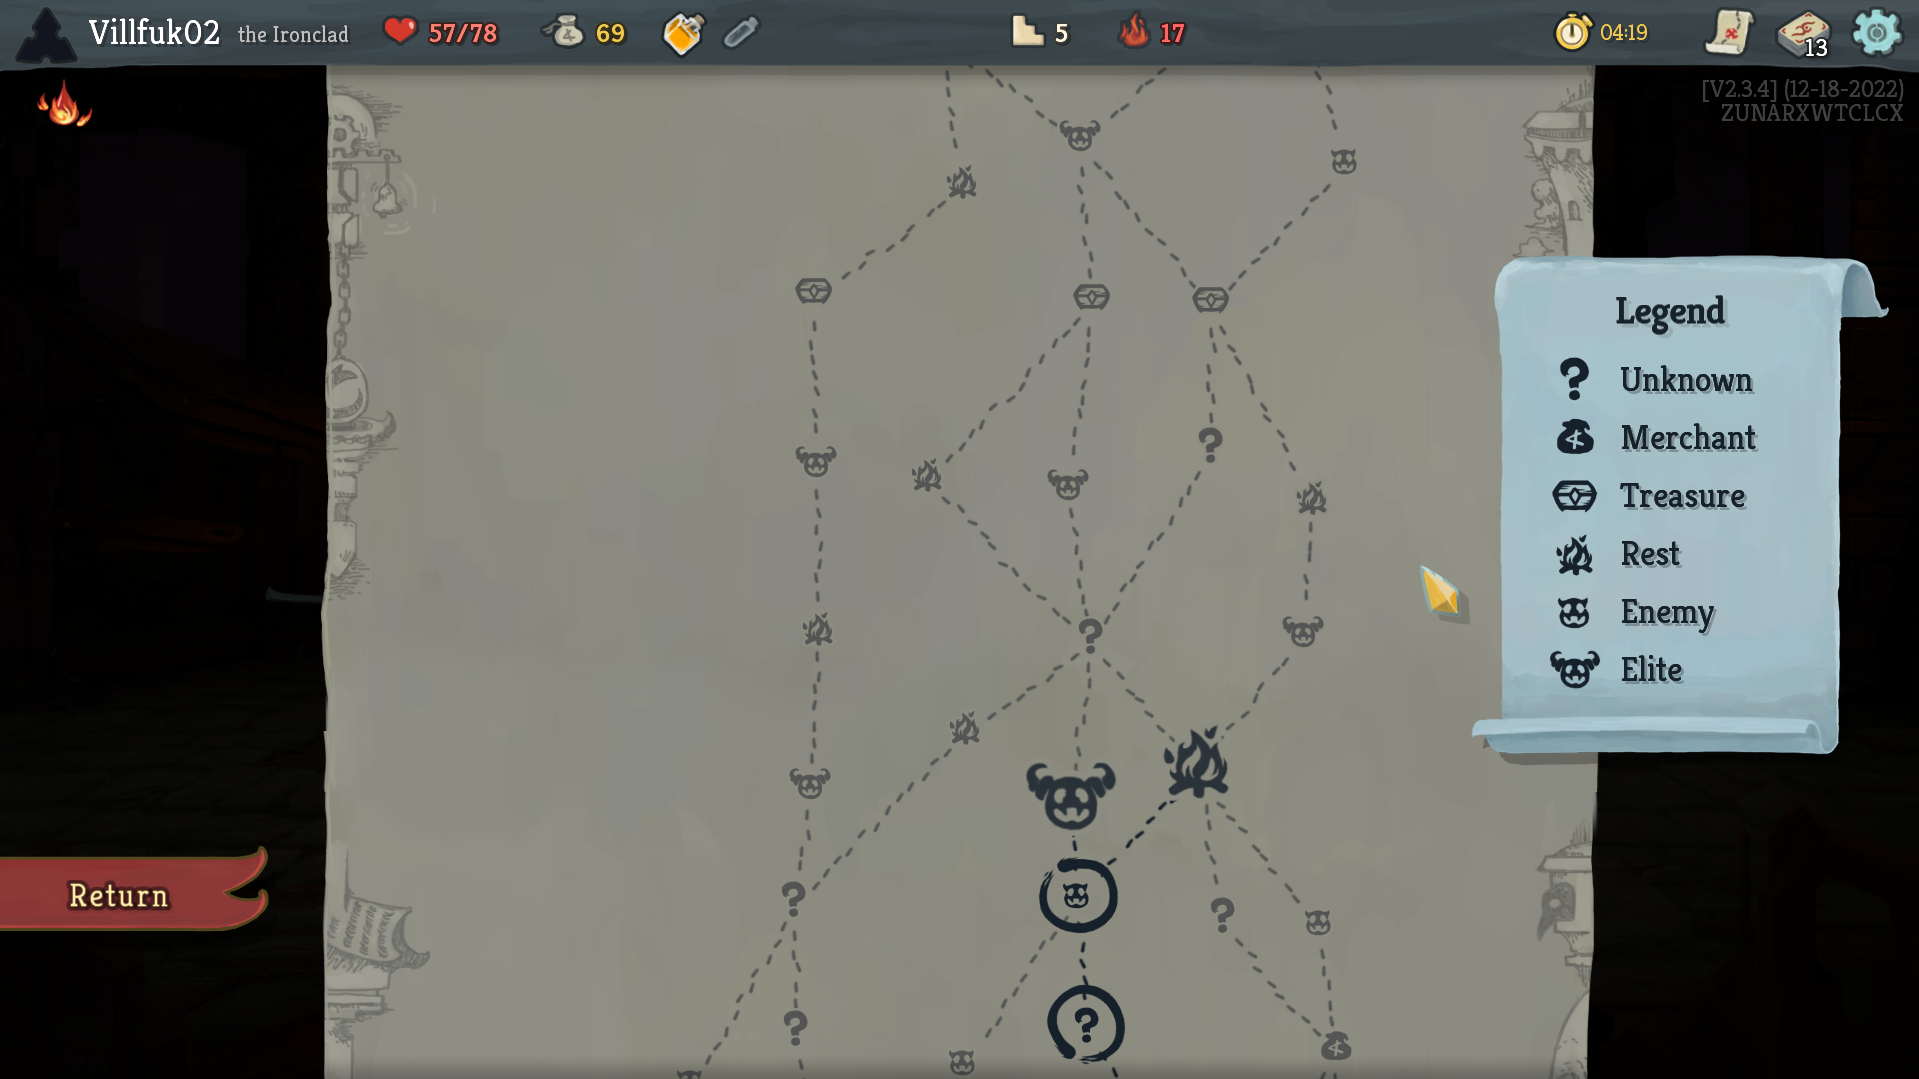
\includegraphics[width=0.8\textwidth]{img/Slay-the-Spire-Map.png}
    \caption{The map screen in \emph{Slay the Spire}.}
    \label{fig:sts-map}
\end{center}

In figure~\ref{fig:sts-fight}, the player character is shown on the left, facing a \emph{Jaw worm} on the right of the screen.
On the bottom, there are cards that the player can play to fight the enemy.
At the start of each turn, the player draws five cards from the deck.
We can see that each card has a name at the top with its corresponding illustration below.
Below the illustration is text explaining the effect of the card when played.
Most cards deal damage to the enemies or provide \emph{block} to defend from enemy attacks, but some have more unique effects.
In the top right corner of a card is displayed its \emph{energy}~cost.
The player can only spend three \emph{energy} per turn, so they can only play a limited amount of the cards they drew.
It is important to play the right cards in order to kill the enemy without taking a lot of damage.

\begin{center}
    \captionsetup{type=figure}
    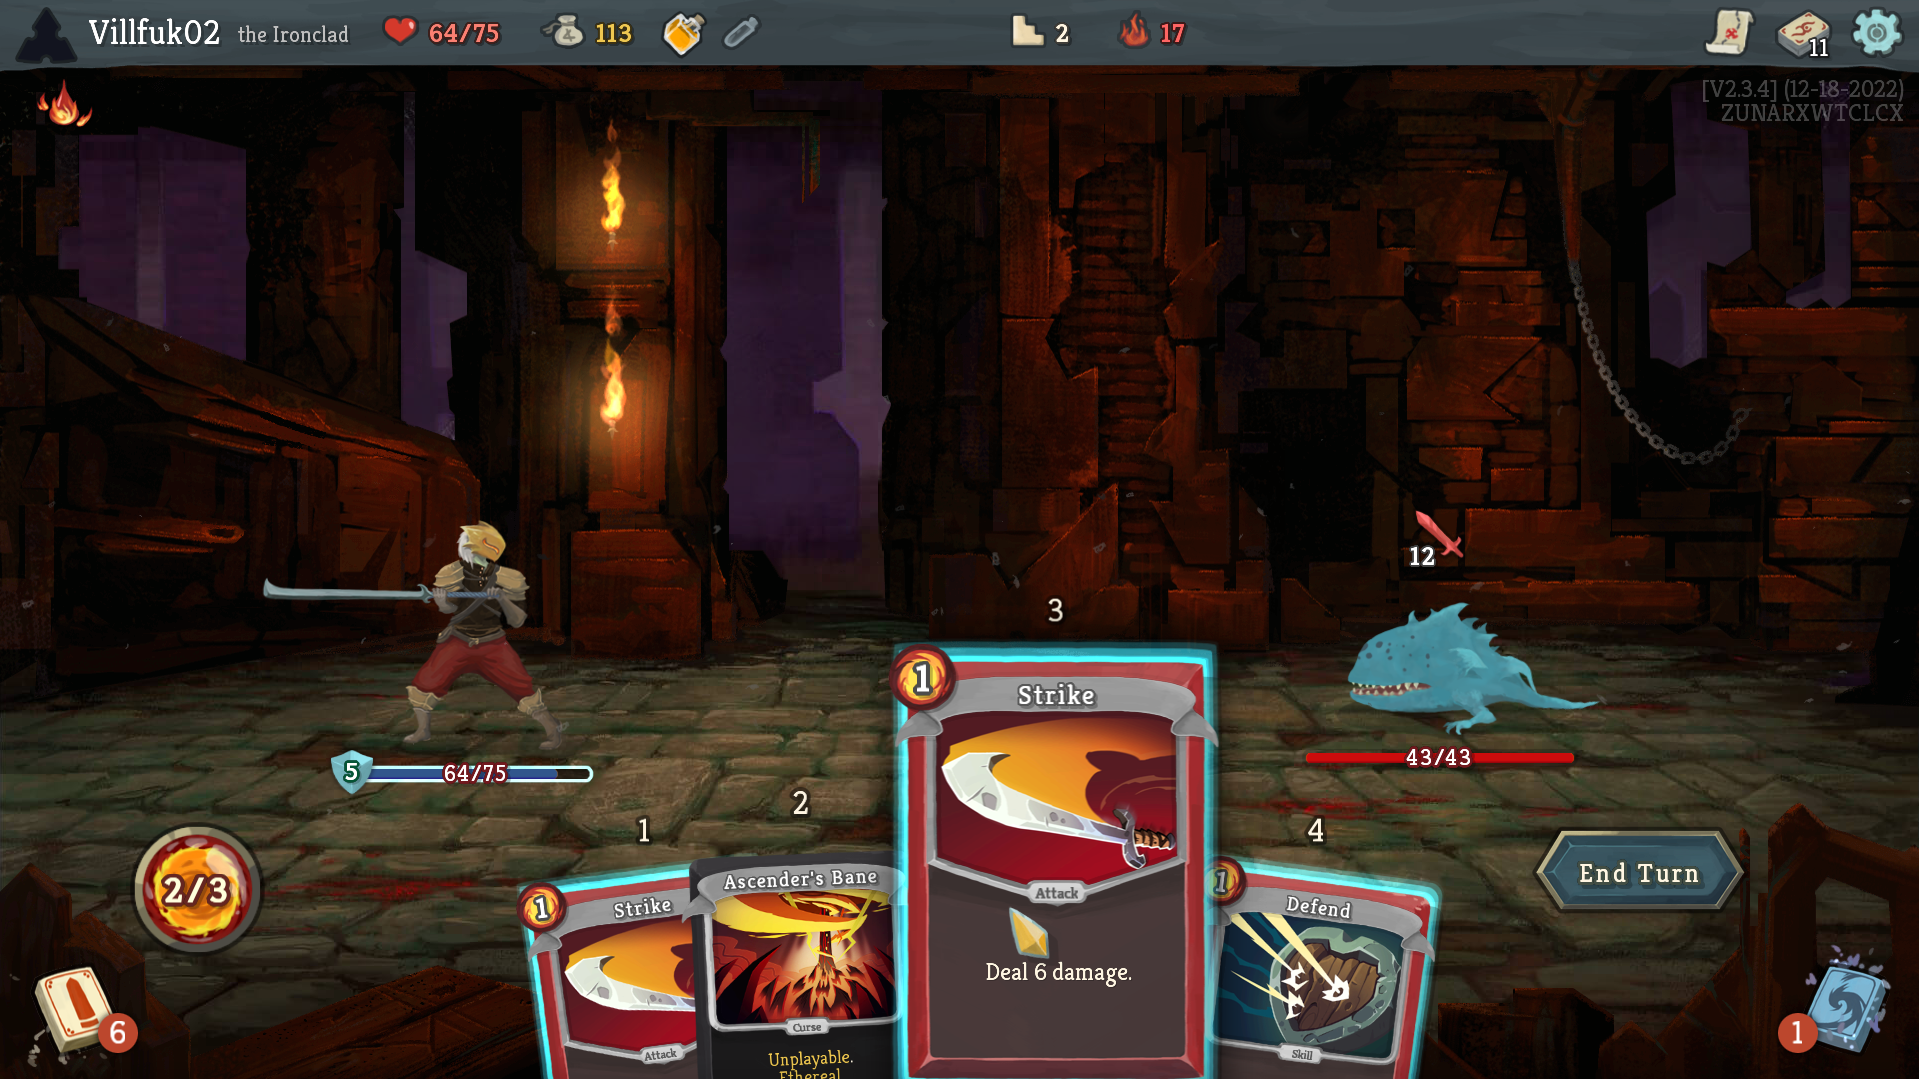
\includegraphics[width=0.8\textwidth]{img/Slay-the-Spire-Fight.png}
    \caption{A fight in \emph{Slay the Spire}.}
    \label{fig:sts-fight}
\end{center}

Even though the player never knows exactly what cards they'll draw, they can shape the deck they draw from throughout the game.
The player starts each run with a predefined deck of starter cards, and as they progress, they add new cards into their deck.
For example, after every fight, they get presented with three randomly selected cards, and they can choose one of them.
The player can also get new cards from events or shops and sometimes remove the cards they don't want.
Some cards are rarer than others, and they are often more powerful.
However, being lucky and getting the most powerful cards is not what the game's about.
The player must learn which cards work together well and which don't, and understand the weaknesses of their deck and how to fix them.

Many games take the \emph{roguelike} mechanic of \emph{permadeath} and randomized procedural generation, but fill in different game mechanics.
\emph{Slay the Spire} has the player build their own deck of cards to play with, but they still play as a character that fights enemies.
Some, however, deviate much more.
In our game, the battles will be in the style of \emph{tower defense}, and the player will collect blueprints for defensive towers and other buildings instead of weapons and armor.

Games that deviate more from the \emph{roguelike} formula are sometimes called \emph{rogueli\textbf{t}e} games.
However, there is no agreement on when a game stops being \emph{roguelike} and starts being \emph{roguelite}.
We will not make this distinction, since game genres have no precise boundaries and can be freely blended with others.

\section{Original Vision} \label{sec:original-vision}

Now that we have introduced the concepts of \emph{tower defense} and \emph{roguelike} games, we can use them to create an overview of the game we intend to make.
It~will be a single-player game.
As stated, the moment to moment gameplay will be a \emph{tower defense}, but on a larger scale, the game will be \emph{roguelike}.
This means that it will consist of individual procedurally generated runs, where the player will start from scratch every time.
During each run, the player will defend against attackers in many battles and improve their arsenal to grow stronger.
Their goal is to get as far as possible, trying to reach the final level and beat the game.

\head{Battles}{ov-battles}
The goal of each battle is to gather enough \emph{fuel} to continue.
The faster the player gathers the \emph{fuel}, the sooner they win the battle.
The \emph{fuel} is generated passively, but additional buildings can be built to speed up the process.
In the meantime, the player has to defend against waves of attackers by building towers and using abilities.
Towers persist throughout the battle and shoot at the attackers, whereas abilities provide single-use effects that can help in a time of need.
All of this costs \emph{materials} and \emph{energy}~--- resources, which are generated by economic buildings.

\head{Procedural generation}{ov-procedural-generation}
Each battle will take place on a unique, procedurally generated terrain.
This means that the paths the attackers take will also differ in each battle.
Furthermore, there will be various kinds of attackers and the attacker waves will also be procedurally generated.

\head{Blueprints}{ov-blueprints}
On their way, the player will choose from randomly selected \emph{blueprints} to add to their collection.
These \emph{blueprints} will allow them to use new abilities, or build new towers and other buildings.
The player will have to choose \emph{blueprints} which work together well in order to use their full potential.

\head{Run progression}{ov-run-progression}
The player will also encounter various shops and events.
These can present additional choices and provide the player with opportunities to gain various rewards or punishments.
The path the player takes will not be linear, allowing them to decide which battles to fight and what to interact with from the map screen.

\head{Platform}{ov-platform}
We will target the game for personal computers only.
Unlike mobile phones, PCs usually have a screen large enough to let us clearly convey all the information the player needs.
It won't be for game consoles either because we think a mouse will be the best way to control the game.
The mouse allows the player to select a precise position in the world quickly.
The player can also control certain aspects of the game using the keyboard.

\section{Current Scope and Goals}\label{sec:thesis-goals}

The scale of the game as outlined in section~\ref{sec:original-vision} is quite large.
Furthermore, it would need a lot of content and polish before being able to be released as a full game.
Instead of creating a full-featured polished game, in this thesis we will focus on making a functional demo version, which can be used to playtest the core gameplay.
The demo will contain some base content in order to be playable, and it must be prepared for future development so that more content can be added later.

The demo version will allow the player to progress through battles and collect blueprints.
However, there will be no map screen to let them choose their path as described in the paragraph \nameref{head:ov-run-progression} of the previous section.
For now, the progression will be linear and there will be no events or shops, only battles.
All the art and sound assets will be placeholders, but care will be taken to make everything as clear as possible to the player.

\hfill\break
The main goals of the thesis are:
\begin{enumerate}
    \item Design the game's mechanics and features.
    \item Implement all the systems and mechanics described in paragraphs \nameref{head:ov-battles}, \nameref{head:ov-procedural-generation} and \nameref{head:ov-blueprints}.
    \item Include a tutorial to explain the game's mechanics to the player.
    \item Conduct a playtest.
\end{enumerate}
